\documentclass[12pt]{article}
\usepackage{verbatim}
\usepackage{graphics}
\usepackage{graphicx}
\usepackage{pstricks,pstricks-add}
\usepackage{amssymb,amsmath}
\newcommand{\FIGUREPATH}{.}

\begin{document}
%to \FIGUREPATH
%\begin{figure}
%\input{walker_on_plane.eps}
%\end{figure}
%\begin{figure}
%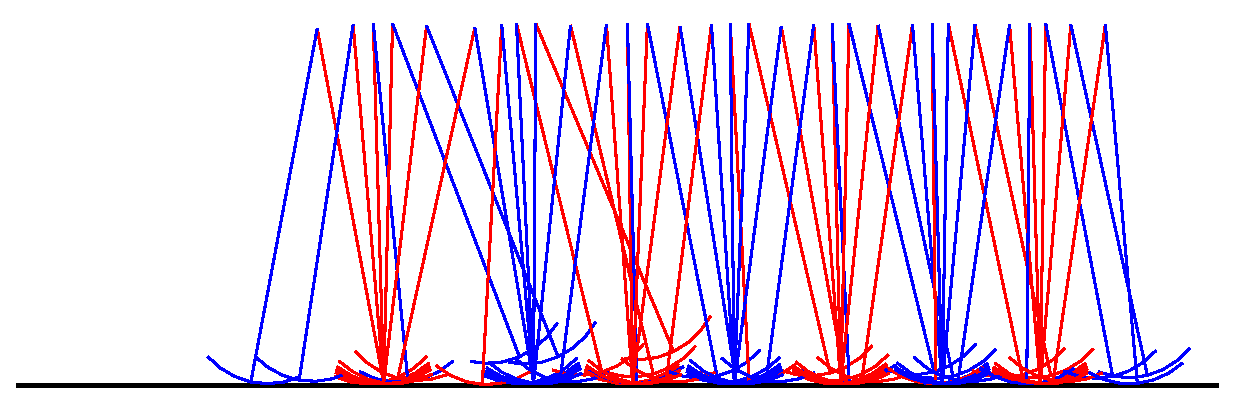
\includegraphics[width=\textwidth]{walker_on_plane.eps}
%\end{figure}

Figures \ref{fig:hello}
\begin{figure}
\documentclass[11pt]{article}
\usepackage{pstricks,pst-eps}
\usepackage{pst-all}
\usepackage{amsmath}
\pagestyle{empty}
\begin{document}
\begin{TeXtoEPS}
\def\Func{y[1]|-y[1]-sin(y[0])}
\psset{unit=1cm,algebraic=true,linewidth=0.5pt}

\begin {pspicture}(-3,-3)(3,3)
\psframe(-2,-2)(2,2)
\psgrid
\psset{method=rk4,plotpoints=400,linecolor=blue,linewidth=1pt,
	whichabs=0,whichord=1}
\multido{\r=0+1}{3}{%
	\psplotDiffEqn{0}{30}{\r\space 0}{\Func}}
\end{pspicture}
\end{TeXtoEPS}
\end{document}


\label{fig:hello}
\end{figure}

\begin{figure}
\documentclass[11pt]{article}
\usepackage{pstricks,pst-eps}
\usepackage{pst-all}
\usepackage{amsmath}
\pagestyle{empty}
\begin{document}
\begin{TeXtoEPS}
\begin{pspicture}(0,0)(10,10)
%\psgrid(0,0)(10,10)(1,1)
\multido{\rA=2+0.25}{16}{
	\psline[linecolor=blue](0,\rA)(10,\rA)
	}
\rput(3,5){
	
	\pspolygon*[linecolor=blue!40](-1,-1)(1,-1)(1.5,2)(-1.5,2)
	\psline{->}(0,-0.5)(0,1.5)
	\psline{->}(-0.5,0)(1.5,0)
	\psline[linecolor=blue,linewidth=2pt]{->}(0,-0.5)(0,-2.5)
	\psdots[dotstyle=Bo,dotscale=1.0,fillcolor=blue](0,-0.5)
	\rput[r](0,-2.5){$\mathbf{g}$}
	\psline[linecolor=red,linewidth=2pt]{->}(0,1)(0,3)
	\psdots[dotstyle=Bo,dotscale=1.0,fillcolor=red](0,1)
	\rput[r](0,3){$\mathbf{b}$}
	\psline[linewidth=0.5pt](0,0)(-2,0)
	\psline[linewidth=0.5pt](0,-0.5)(-2,-0.5)
	\psline[linewidth=0.5pt]{<->}(-1,0)(-1,-0.5)
	\rput(-2.2,0.25){ $\mathbf l_{g}$}	
	
	\psline[linewidth=0.5pt](0,0)(2,0)
	\psline[linewidth=0.5pt](0,1)(2,1)
	\psline[linewidth=0.5pt]{<->}(1,0)(1,1)
	\rput(2.2,0.5){$\mathbf l_{b}$}	
	

	}
\rput{10}(7,5){
		\pspolygon*[linecolor=blue!40](-1,-1)(1,-1)(1.5,2)(-1.5,2)
		\psline[linewidth=0.5pt]{->}(0,-0.5)(0,1.5)
		\psline[linewidth=0.5pt]{->}(-0.5,0)(2,0)
		\psarc[linewidth=0.5pt]{->}(0,0){1.8}{-10}{0}
			\rput{-10}(0,0)
			{
			\psline{->}(0,-0.5)(0,1.5)
			\psline{->}(-0.5,0)(2,0)
			\rput(2,0){$\mathbf{q}$}	
			}
		\rput{-10}(0,1)
		{
		\psdots[dotstyle=Bo,dotscale=1.0,fillcolor=red](0,0)
		\psline[linecolor=red,linewidth=2pt]{->}(0,0)(0,2)
		\rput[r](0,2){$\mathbf{b}$}
		}
		
		\rput{-10}(0,-0.5)
		{
		\psdots[dotstyle=Bo,dotscale=1.0,fillcolor=blue](0,0)
		\psline[linecolor=blue,linewidth=2pt]{->}(0,0)(0,-2)
		\rput[r](0,-2){$\mathbf{g}$}
		}
		
		}

\end{pspicture}
\end{TeXtoEPS}
\end{document}
%% \multido{\rA=0.00+0.25}{12}{\pslineByHand[linecolor=blue](0,\rA)(\linewidth,\rA)}



\end{figure}

\begin{figure}
\begin{center}
\begin{pspicture}(0,0)(10,10)
%\psgrid(0,0)(10,10)(1,1)
\multido{\rA=2+0.25}{16}{
\psline[linecolor=blue](0,\rA)(10,\rA)
	}

\rput(3,5){
	\pspolygon*[linecolor=blue!40](-1,-1)(1,-1)(1.5,2)(-1.5,2)
		\rput(0,1)
		{
		\psdots[dotstyle=Bo,dotscale=2.0,fillcolor=red](0,0)
		\psline[linecolor=red,linewidth=2pt]{->}(0,0)(0,2)
		\rput[r](0,2){$\mathbf{b}$}
		}
		
		\rput(0,-0.5)
		{
		\psdots[dotstyle=Bo,dotscale=2.0,fillcolor=blue](0,0)
		\psline[linecolor=blue,linewidth=2pt]{->}(0,0)(0,-2)
		\rput[r](0,-2){$\mathbf{g}$}
		}
	}

\rput(7,5){
	\rput{180}(0,1.2){
	\pspolygon*[linecolor=blue!40](-1,-1)(1,-1)(1.5,2)(-1.5,2)
	}
		\rput(0.05,0.8)
		{
		\psdots[dotstyle=Bo,dotscale=2.0,fillcolor=red](0,0)
		\psline[linecolor=red,linewidth=2pt]{->}(0,0)(0,2)
		\rput[r](0,2){$\mathbf{b}$}
		}
		
		\rput(-0.05,1.5)
		{
		\psdots[dotstyle=Bo,dotscale=2.0,fillcolor=blue](0,0)
		\psline[linecolor=blue,linewidth=2pt]{->}(0,0)(0,-2)
		\rput[r](0,-2){$\mathbf{g}$}
		}
		
	}
\end{pspicture}
\end{center}


\end{figure}

\begin{figure}
\begin{center}
\def\Func{y[1]|-y[1]-sin(y[0])}
\psset{unit=1.5cm,algebraic=true,linewidth=0.5pt}

\begin {pspicture}(-3,-3)(3,3)
\psframe(-1,-1)(1,)
\psaxes{->}(0,0)(-2,-2)(2,2)

\psset{method=rk4,plotpoints=20,linecolor=blue,linewidth=1pt,
	whichabs=0,whichord=1,arrows=->,ArrowInside=->,arrowscale=0.7}
\multido{\row=-1+0.2}{10}{%
	\psplotDiffEqn{0}{5}{\row\space -1}{\Func}
	\psplotDiffEqn{0}{5}{\row\space 1}{\Func}
	\psdots[dotstyle=Bo,dotscale=0.5,fillcolor=red](\row,-1)
	\psdots[dotstyle=Bo,dotscale=0.5,fillcolor=red](\row,1)
	}
\multido{\row=-1+0.2}{10}{%
	\psplotDiffEqn{0}{5}{-1 \row}{\Func}
	\psplotDiffEqn{0}{5}{1 \row}{\Func}
	\psdots[dotstyle=Bo,dotscale=0.5,fillcolor=red](-1,\row)
	\psdots[dotstyle=Bo,dotscale=0.5,fillcolor=red](1,\row)
	}
	
\psdots[dotstyle=Bo,dotscale=2.0,fillcolor=red](0,0)		
\end{pspicture}
\end{center}


\end{figure}

\begin{figure}
\documentclass[11pt]{article}
\usepackage{pstricks,pst-eps}
\usepackage{pst-all}
\usepackage{amsmath}
\pagestyle{empty}
\begin{document}
\begin{TeXtoEPS}
\def\Func{y[1]|-2*y[1]-sin(y[0])}
\psset{unit=10cm,algebraic=true,linewidth=0.5pt}

\begin {pspicture}(-3.5,-0.5)(-2.7,0.5)
%\psgrid
\psframe(-3.24,-0.1)(-3.04,0.1)

\psaxes[labels=none]{->}(-3.14159265357,0)(-3.5,-0.3)(-2.7,0.3)
\psset{method=rk4,plotpoints=10,linecolor=blue,linewidth=1pt,
	whichabs=0,whichord=1,arrows=->,ArrowInside=->}
\psdots[dotsize=1cm](0,0)
\multido{\row=-3.24+0.1}{3}{%
	\psplotDiffEqn{0}{3}{\row\space -0.1}{\Func}
	\psplotDiffEqn{0}{3}{\row\space 0.1}{\Func}
	\psdots[dotstyle=Bo,dotscale=0.5,fillcolor=red](\row,-0.1)
	\psdots[dotstyle=Bo,dotscale=0.5,fillcolor=red](\row,0.1)
	}
\multido{\row=-0.1+0.025}{5}{%
	\psplotDiffEqn{0}{3}{-3.04 \row}{\Func}
	\psplotDiffEqn{0}{3}{-3.24 \row}{\Func}
	\psdots[dotstyle=Bo,dotscale=0.5,fillcolor=red](-3.04,\row)
	\psdots[dotstyle=Bo,dotscale=0.5,fillcolor=red](-3.24,\row)
	}

\psdots[dotstyle=Bo,dotscale=2.0,fillcolor=red](-3.14159265357,0)
\end{pspicture}
\end{TeXtoEPS}
\end{document}



\end{figure}

\begin{figure}
\documentclass[11pt]{article}
\usepackage{pstricks,pst-eps}
\usepackage{pst-all}
\usepackage{amsmath}
\pagestyle{empty}
\begin{document}
\begin{TeXtoEPS}
\def\Func{y[1]|-y[1]-sin(y[0])}
\psset{algebraic=true,linewidth=0.5pt}

\begin {pspicture}(-3.5,-1)(2,2)
\psaxes[labels=none,ticks=none]{->}(0,0)(-3.5,-1)(2,2)
\psset{method=rk4,plotpoints=400,linecolor=blue,linewidth=1pt,
	whichabs=0,whichord=1}
\multido{\row=-3+0.2}{3}{%
	\psplotDiffEqn{0}{30}{\row\space 0.1}{\Func}
	\psdots[dotstyle=Bo,dotscale=0.5,fillcolor=red](\row,0.1)
	}
\multido{\row=0.1+0.1}{4}{%
	\psplotDiffEqn{0}{30}{-3.14 \row}{\Func}
	\psdots[dotstyle=Bo,dotscale=0.5,fillcolor=red](-3.14, \row)
	}
\psdots[dotstyle=Bo,dotscale=1.0,fillcolor=red](-3.14159265357,0)
\psdots[dotstyle=Bo,dotscale=1.0,fillcolor=black](0,0)
\end{pspicture}
\end{TeXtoEPS}
\end{document}


\end{figure}

\begin{figure}
\begin{center}
\begin {pspicture}(-3,-3)(3,3)
\psarc[linewidth=2pt](0,0){2}{0}{360}
\psdots[dotstyle=Bo,dotscale=3,fillcolor=red](-2,0)
\rput[r](-2,0){Unstable Equilibrium}
\psdots[dotstyle=Bo,dotscale=3,fillcolor=blue](2,0)
\rput[l](2,0){Stable Equilibrium}
\psarc{<-}(0,0){2.5}{60}{120}
\psarc{->}(0,0){2.5}{-120}{-60}
\end{pspicture}
\end{center}


\end{figure}


\begin{figure}
\begin{center}
\psset{whichabs=0,whichord=1}
\begin{pspicture}(0,0)(10,10)
%\psgrid(0,0)(10,10)(1,1)
\rput(5,5){
	\multido{\rA=-2+0.25}{20}{\psline[linecolor=blue](-5,\rA)(!-4 \rA \space 0.5 add)(-3,\rA)(5,\rA)}
	\rput{90}(0,0){\pspolygon*[linecolor=blue](-1,-1)(-2,0)(-1,1)(3,1)(3,-1)
			\psline[linewidth=2pt]{->}(0,0)(-3,0)	}
	\pspolygon*[linecolor=blue!40](-1,-1)(-2,0)(-1,1)(3,1)(3,-1)
	\psline[linewidth=2pt]{->}(0,0)(-3,0)
	\psarc{<-}(0,0){3.3}{180}{270}
	\SpecialCoor
	\rput[r](3;225){Stir}
}

\end{pspicture}
\end{center}


\end{figure}

\begin{figure}
\begin{center}
\begin{pspicture}(0,0)(10,10)
%\psgrid(0,0)(10,10)(1,1)
\multido{\rA=2+0.25}{16}{
	\psline[linecolor=blue](0,\rA)(10,\rA)
	}
\rput(6,5){\pspolygon*[linecolor=blue!40](-2,2)(-1,-1)(3,-1)(3,2)
	}
\rput(2,5){\pspolygon*[linecolor=blue](-1,-1)(1,-1)(1.5,2)(-1.5,2)}
\end{pspicture}
\end{center}


\end{figure}

\begin{figure}
\begin{center}
\def\Func{y[1]|-0.5*y[1]-0.5*sin(y[0])}
\def\Funcc{y[1]|-y[1]-sin(y[0])}
\psset{unit=1cm,algebraic=true,linewidth=0.5pt}
\begin {pspicture}(-2.5,-2.5)(2.5,2.5)
\rput(3,0){
\psgrid(0,0)(-2,-2)(2.2,2)
\psset{method=rk4,plotpoints=400,linecolor=blue,linewidth=1pt,
	whichabs=0,whichord=1}
\multido{\r=0.5+0.5}{2}{%
	\psplotDiffEqn{0}{30}{\r\space 0}{\Func}
	\psdots[dotstyle=Bo,dotscale=0.5,fillcolor=red](\r,0)
	}

}
\rput(-3,0)
{

\psgrid(0,0)(-2,-2)(2.2,2)
\psset{method=rk4,plotpoints=400,linecolor=blue,linewidth=1pt,
	whichabs=0,whichord=1}
\multido{\r=1+1}{2}{%
	\psplotDiffEqn{0}{30}{\r\space 0}{\Funcc}
	\psdots[dotstyle=Bo,dotscale=0.5,fillcolor=red](\r,0)
	}
	
}
\end{pspicture}
\end{center}


\end{figure}

\end{document}


\begin{comment}
bb_ms_os_Phase.eps
bb_ms_os_StateTimeAttraction.eps
bb_ms_os_StateTime.eps
bouncing_ball.eps
bouncing_ball_phaseplot.eps
duffin.eps
entraint_oscilation.eps
mass_neural_entraint.eps
mass_neural_mass_phase.eps
mass__neural_oscilation_phase.eps
mass_oscilation_attraction_phase.eps
mass_spring.eps
massspring.eps
mass_state_attraction_phase.eps
mass_state.eps
neural1phase.eps
neural_attraction.eps
neuraloscilation1.eps
oscilation.eps
pendulum.eps
spring_damping.eps
\end{comment}
